%=========================================================================================================

\documentclass[11pt,letterpaper]{article}

%% arquivo de definições de estilo documento
%==========================================================================================
% Pacotes

%% definições relacionadas a idioma
\usepackage[brazil]{babel}

%% codificação de caracteres
%% http://tex.stackexchange.com/questions/664/why-should-i-use-usepackaget1fontenc
%% http://tex.stackexchange.com/questions/44694/fontenc-vs-inputenc
\usepackage[T1]{fontenc}
\usepackage[utf8]{inputenc}    % usar se salvar com codificação UTF-8
%\usepackage[latin1]{inputenc}  % usar se salvar com codificação ISO

%% definições das margens
\usepackage[top=4.5cm,left=4.5cm,right=4.5cm,bottom=4.5cm]{geometry}

%% para inserir figuras em diversas extensões
\usepackage{graphicx}

%% controla o uso de Teorema, Definição, Exemplo, Demonstração, Exercício
\usepackage{amsthm}

%% todos os pacotes da AMS (American Mathematical Society), inúmeros símbolos
\usepackage{amsfonts,amssymb,amsxtra,empheq}  
\usepackage[mathscr]{eucal}

%% permite o uso de vírgula como separador decimal no ambiente matemático
\usepackage{icomma} 

%% permite o uso de comentários entre \begin{comment}...\end{comment}                 
\usepackage{comment}

%% cores em palavras, frases, etc. \textcolor{red}{text in red}
\usepackage{color}

%% permite a indentação do 1º paragráfo após um título de seção, capítulo
\usepackage{indentfirst}
%%%% recuo da primeira linha de cada parágrafo
  %\setlength{\parindent}{1.2cm}

%% permite a construção do texto colunas
\usepackage{multicol}

%% controla o espaçamento entre linhas
\usepackage{setspace}
%%%% espaçamento 1.5 linha no texto \begin{spacing}{1.0}...\end{spacing}
  \onehalfspace                      

%% permite desenhar
%% http://www.texample.net/tikz/
%\usepackage{tikz}
%\usetikzlibrary{decorations.pathreplacing}
%\usetikzlibrary{arrows,decorations.pathmorphing}
%\usetikzlibrary{shapes,backgrounds}  
  
%% para colocar a legenda indentada como formato da UFLA
\usepackage[format=hang, labelsep=quad]{caption}

%% controla objetos flutuantes e permite definir novas classes
%% útil para criar a classe de fluantes 'program', para código
\usepackage{float}
%%%% algumas formas de denifir
%   \floatstyle{ruled}
%   \newfloat{Input}{tbp}{lop}[section]
%   \floatname{Input}{Program}

%% controla novos ambientes que listam índices, e.g. lista de anexos
\usepackage{listings}

%% texto em caixas
\usepackage{boxedminipage}

%% controle e definição de ambientes numerados
%% listas mais compactas, úteis para salvar espaço
%% http://tex.stackexchange.com/questions/62009/paralist-environment
\usepackage{paralist}

%% para rotacionar tabela \begin{sidewaystable}
\usepackage{rotating} 

%% rotacionar texto \begin{landscape}
\usepackage{lscape} 

%% para ter tabelas com linhas mescladas
\usepackage{multirow}

%% para inserir epigrafe
\usepackage{epigraph}

%% notas de rodapé
\usepackage[symbol, hang, flushmargin]{footmisc} 

% controle e definições para tamanho de colunas em tabelas
\usepackage{array} 
\newcolumntype{C}[1]{>{\centering\let\newline\\\arraybackslash\hspace{0pt}}m{#1}}
\newcolumntype{R}[1]{>{\raggedleft\let\newline\\\arraybackslash\hspace{0pt}}m{#1}}

%==========================================================================================
% Definições

%% redefine o espaçamento entre linhas
\renewcommand{\baselinestretch}{1.2cm}
\def\onehalspacing{1.5}

%% permite leitura do caracter @ nas definições que seguem
\makeatletter

%%.....................................................
%% Sessões

%% definição do texto título da sessão
\renewcommand{\section}{\@startsection
{section}%                     % the name
{1}%                           % the level
{0mm}%                         % the indent
{-\baselineskip}%              % the before skip
{1.\baselineskip}%             % the after skip
{\noindent\normalsize\textbf}} % the style

%% definição do texto título da subsessão
\renewcommand{\subsection}{\@startsection
{subsection}%                  % the name
{2}%                           % the level
{0mm}%                         % the indent
{-\baselineskip}%              % the before skip
{0.1\baselineskip}%            % the after skip
{\noindent\normalsize\textbf}} % the style
\makeatother

%% desabilita o uso do @
\makeatother

%%.....................................................
%% Sumário

%% sumário alinhado à esquerda
\usepackage{titletoc}
\def\distnumber{2.3em}

\titlecontents{section}       % set formatting for \section
[\distnumber]                 % adjust left margin
{\bfseries}                   % font formatting
{\contentslabel{\distnumber}} % section label and offset
{\hspace*{-\distnumber}}
{\normalfont\titlerule*[1pc]{.}\contentspage}

\titlecontents{subsection}    % set formatting for \section
[\distnumber]                 % adjust left margin
{\bfseries}                   % font formatting
{\contentslabel{\distnumber}} % section label and offset
{\hspace*{-\distnumber}}
{\normalfont\titlerule*[1pc]{.}\contentspage}

\setcounter{tocdepth}{4}
\renewcommand{\baselinestretch}{1.5} % espaçamento entre linha
\numberwithin{equation}{section}     % numerar equação por seção

%%.....................................................
%% Flutuantes e equações

%% nomes
\renewcommand{\figurename}{Figura}
\renewcommand{\tablename}{Tabela}

%% profundidade de numeração
%\numberwithin{figure}{section}
%\numberwithin{table}{section}
%\numberwithin{equation}{section}

%%.....................................................
%% Paginação

\usepackage{fancyhdr}
\renewcommand{\headrulewidth}{0pt}
\fancyhf{}
\fancyhead[R]{\thepage}

%%.....................................................
%% Fontes

%% fonte para o texto
\usepackage{times}

%% fonte para ambiente matemático mais parecido com Times
\usepackage{txfonts}

%% fonte para ambiente de código (monospaced)
\usepackage[scaled=0.85]{beramono}

%%.....................................................
%% Referências e hyperlinks

\usepackage{hyperref} %transformas o sumário e as citações em hiperlinks
\hypersetup{
%    bookmarks=true,         % show bookmarks bar?
%    unicode=false,          % non-Latin characters in Acrobat's bookmarks
%    pdftoolbar=true,        % show Acrobat's toolbar?
%    pdfmenubar=true,        % show Acrobat's menu?
%    pdffitwindow=true,      % page fit to window when opened
  pdftitle={Parametrizações interpretáveis em modelos não lineares},
  pdfauthor={Walmes Marques Zeviani},
  pdfsubject={Tese de Doutorado},
  pdfcreator={Walmes Marques Zeviani},
  pdfproducer={Walmes Marques Zeviani},
  pdfkeywords={Verossimilhança, Curvatura, Método delta, van Genuchten},
%    pdfnewwindow=true,      % links in new window
  colorlinks=true,           % false: boxed links; true: colored links
  linkcolor=black,           % color of internal links
  citecolor=black,           % color of links to bibliography
  filecolor=red,             % color of file links
  urlcolor=cyan              % color of external links
}

%%.....................................................
%% Comandos

\newcommand{\lin}{\noindent \rule[4mm]{\textwidth}{0.1ex}}

%==========================================================================================


%% para referencias bibliográficas no padrão ABNT
\usepackage[abnt-substyle=UFLA,abnt-emphasize=bf,abnt-etal-list=3,abnt-and-type=e]{abntcite}

%=========================================================================================================
% Definições de conteúdo

%% título em português e inglês e caixa alta
\def\tesetitle{Parametrizações interpretáveis em modelos não lineares}
\def\tesetitleeng{Interpretable parametrization in nonlinear models}
\def\tesetitlecap{\expandafter\MakeUppercase\expandafter{\tesetitle}}

%% autor e abreviações
\def\teseauthor{Walmes Marques Zeviani}
\def\teseauthorcap{\expandafter\MakeUppercase\expandafter{\teseauthor}}
\def\teseauthorrev{Zeviani, Walmes Marques}
\def\teseauthorcrv{ZEVIANI, Walmes Marques}

%% ano
\def\teseyear{2013}

%% orientador
\def\teseorientador{Joel Augusto Muniz}

%% palavras com infenização manual (não contidas no dicionário)
\hyphenation{ne-ces-s\'arias fa-zen-do pa-r\^{a}-me-tro a-va-li-ar vi-san-do pr\'o-prias
              Ge-nu-chten fi-ca-ram a-do-\c{c}\~ao in-ter-pre-t\'a-veis mo-no-mo-le-cu-lar
              re-pa-ra-me-tri-z\'a-lo}

\begin{document}
\pagestyle{empty}

%=========================================================================================================

%% inclui as capas, folhas de rosto, etc
%=========================================================================================================
% capa

\setcounter{page}{0}
\thispagestyle{empty}
\section*{}
\vspace{-0.7cm}
\begin{singlespace}
\begin{center}

\includegraphics[width=4cm]{../figuras/UFLAlogo}\\
\vspace{.6cm}
\Large{\textbf{\teseauthorcap}}
\end{center}

\vfill

\vspace{-0.5cm}
\begin{center}
\begin{minipage}{10cm}
\begin{center}
\Large{\textbf{\tesetitlecap}} 
\end{center}
\end{minipage}
\end{center}

\vfill
\begin{center}
{\textbf{LAVRAS - MG\\ \teseyear}}
\end{center}
\end{singlespace}

% página em branco
\newpage\null\thispagestyle{empty}\newpage

%=========================================================================================================
% folha de rosto

\newpage
%\section*{}
\vspace{-0.7cm}
\centerline{\textbf{\teseauthorcap}}
\vspace{1.4cm}
\begin{singlespace}
\begin{center}
\textbf{\tesetitlecap}
\end{center}
\end{singlespace}
\vspace{1cm}
\begin{flushright}
\begin{minipage}{9.6cm}
\begin{quote}
\begin{singlespace}
Tese apresentada à Universidade Federal de Lavras, como parte das exigências do Programa de Pós-Graduação em Engenharia Florestal, área de concentração em Manejo Florestal, para a obtenção do título de Doutor.
\end{singlespace}
\end{quote}
\end{minipage}
\end{flushright}
\vspace{1.1cm}

\begin{center}
\begin{singlespace}
\noindent Orientador\\
\noindent Prof. Dr. \teseorientador

\vfill

\Large{\textbf{LAVRAS - MG\\ \teseyear}}
\end{singlespace}
\end{center}

%=========================================================================================================
% ficha catalográfica

\newpage
\textcolor{white}{fantasma}

\vfill
\begin{center}
\begin{singlespace}
\large{\textbf{
Ficha Catalográfica Preparada pela Divisão de Processos Técnicos da Biblioteca da UFLA
}}
\vspace{-1cm}
\end{singlespace}
\end{center}
\begin{center}
\begin{boxedminipage}{12.8cm}
\begin{singlespace}
\begin{center}
\hspace*{0.8cm}
\begin{tabular}{p{11cm}}
\vspace{0.5cm} \noindent{\teseauthorrev.}\\
\hspace*{0.5cm} \tesetitle{} / \teseauthor.  -- Lavras : UFLA, \teseyear.\\
\hspace*{0.5cm} \pageref{ultima} p. : il.
\vspace{0.4cm}

\hspace{0.5cm} Tese (doutorado) -- Universidade Federal de Lavras, \teseyear.\\
\hspace{0.5cm} Orientador: \teseorientador.\\
\hspace{0.5cm} Bibliografia.

\vspace{0.4cm}

\hspace{0.8cm} 1. Verossimilhança. 2. Método delta. 3. Medida de curvatura.
4. Efeitos mistos. 5. van Genuchten. I. Universidade Federal de Lavras. II. Título.\\
\multicolumn{1}{r}{}\\
\multicolumn{1}{r}{CDD-519.76}
\end{tabular}
\end{center}
\end{singlespace}
\end{boxedminipage}
\end{center}
\pagebreak[4]

%=========================================================================================================
% página de aprovação

\newpage
%\section*{}
\vspace{-0.7cm} \centerline{\textbf{\teseauthorcap}}
\vspace{1.4cm}
\begin{singlespace}
\begin{center}
\textbf{\tesetitlecap}
\end{center}
\end{singlespace}
\vspace{0.5cm}

\begin{flushright}
\begin{minipage}{9.6cm}
\begin{quote}
\begin{singlespace}
Tese apresentada à Universidade Federal de Lavras, como parte das 
exigências do Programa de Pós-Graduação em Estatística e 
Experimentação Agropecuária, área de concentração em Estatística e 
Experimentação Agropecuária, para a obtenção do título de Doutor.
\end{singlespace}
\end{quote}
\end{minipage}
\end{flushright}
\vspace{1cm}

\noindent\begin{tabular}{ll}
APROVADA em 13 de maio de 2013.\\
Prof. Dr. Paulo Justiniano Ribeiro Jr & UFPR\\
Prof. Dr. Júlio da Motta Singer & IME-USP\\
Prof. Dr. Júlio Silvio de Sousa Bueno Filho & UFLA\\
Prof. Dr. Augusto Ramalho de Morais & UFLA
\end{tabular}

\begin{center}
\begin{singlespace}
\vspace{0.8cm}
\centerline{Prof. Dr. \teseorientador}
\centerline{Orientador}
\vfill
{\textbf{LAVRAS - MG\\ \teseyear}}
\end{singlespace}
\end{center}

% página em branco
\newpage\null\thispagestyle{empty}\newpage

%=========================================================================================================
% dedicatória

\vspace{1cm}
\begin{flushright}

\textit{\textbf{À DEUS, autor da minha vida.}\
\hspace{15cm} Aos meus pais, Jaime e Marilene, por todo amor, cuidado,
\hspace{13cm} apoio, respeito, confiança e paciência;}

\textit{Aos meus irmãos, Wolnei e Waires, pela admiração, respeito e amizade.}
 
\hspace{15cm}\textbf{DEDICO}
\end{flushright}

% página em branco
\newpage\null\thispagestyle{empty}\newpage

%===============================================================================
% agradecimentos

\newpage
\begin{center}
\textbf{AGRADECIMENTOS}
\end{center}
\vspace{0.5cm}

À meu pai, Roberto e a minha mãe, Vera, por todo carinho, 
apoio.

(omitido)

À UFLA pela oportunidade 
Ao IFSULDEMINAS

À CAPES e ao CNPq pela bolsa de Doutorado.

%===============================================================================
% epigrafe

\newpage
\section*{}
\vspace{8cm}

\setlength{\epigraphrule}{0pt}
\epigraph{
``Experiência não é o que acontece com você, mas o que você fez com o que lhe 
aconteceu.''}{Aldous Huxley}

\setlength{\epigraphrule}{0pt}
\epigraph{
``O que você sabe não tem valor, o valor está no que você faz com o
que sabe.''}{Bruce Lee}
 
\setlength{\epigraphrule}{0pt}
\epigraph{
``Quem não sabe o que busca não identifica o que acha.''}{Immanuel Kant}

% página em branco
\newpage\null\thispagestyle{empty}\newpage

%===============================================================================


%=========================================================================================================

\newpage
\pagestyle{empty}

%% inclui resumo e abstract geral
%=========================================================================================================
% Resumo

\begin{singlespace}
\begin{center}
\section*{RESUMO GERAL}
\end{center}

Uma das vantagens dos modelos de regressão não linear é ter
interpretação para os parâmetros. Em muitas situações, parâmetros de
interesse, expressos como função dos parâmetros do modelo, são
quantidades sujeitas à investigação. Surge então a preocupação de como
fazer inferência sobre eles. Para isso, o método delta, a simulação
Monte Carlo e procedimentos bootstrap são alternativas
frequentes. Além disso, uma reparametrização pode ser aplicada ao
modelo de forma à representar tais parâmetros de interesse. Além de
melhorar a interpretação, a presença do parâmetro alvo estende as
possibilidades com relação a especificação de modelos e inferência
estatística. O objetivo com esse trabalho é sistematizar o
procedimento de aplicar reparametrizações. Ênfase foi dada em modelos
não lineares considerados em aplicações dentro das Ciências
Agrárias. Uma lista com 17 modelos reparametrizados é fornecida. No
primeiro estudo de caso, o nível de dano econômico da desfolha no
algodoeiro foi avaliado com os seguintes objetivos: 1) propor uma
parametrização de modelo que representasse o nível de dano econômico,
2) avaliar parametrizações alternativas por meio de suas propriedades,
onde considerando medidas de não linearidade, 3) aplicar inferência
baseada em verossimilhança, 4) selecionar um modelo para descrever a
relação entre produção e desfolha do algodoeiro em função do estágio
fenológico. O modelo reparametrizado apresentou melhores propriedades
nos estágios fenológicos com pronunciada relação não linear. No
restante, as medidas de curvatura, as correlações dos estimadores e os
gráficos de perfil de verossimilhança indicaram que um sub-modelo
deveria ser considerado. No segundo estudo de caso, objetiva-se
verificar o efeito da posição de amostragem e profundidade do solo
sobre os parâmetros $I$ (\emph{infletion}) e $S$ (\emph{slope}) da
curva de retenção de água do solo. Para isso 1) considerou-se ANOVA
simples e 2) ANOVA ponderada pela variância das estimativas desses
parâmetros em cada unidade experimental em comparação com 3) o uso de
modelos não lineares de efeitos mistos em uma parametrização
desenvolvida. Nenhum dos métodos alternativos de análise foi superior
ao modelo não linear de efeitos mistos na parametrização desenvolvida,
que apresentou intervalos de confiança mais estreitos para os
parâmetros e apontou efeito de posição e profundidade de coleta.\\
\newline
\noindent {Palavras-chave:} Verossimilhança. Método delta. Medidas de
curvatura. Efeitos mistos. van Genuchten.
\end{singlespace}

%=========================================================================================================
% Abstract

\newpage
\begin{singlespace}
\begin{center}
\section*{GENERAL ABSTRACT}
\end{center}

One of the advantages of the nonlinear regression models is to have
interpretable parameters. In many instances, the parameters of
interest, expressed as a function of the model parameters, are
quantities subject to investigation. Then comes the concern of how to
make inferences about them. For this, the delta method, the Monte
Carlo simulation and bootstrap procedures are common alternatives. In
addition, a reparametrization can be applied to the model in order to
represent these parameters of interest into the model. In addition to
improving the interpretation of the presence of the target parameter
extends the possibilities regarding the specification of models and
statistical inference. The aim of this work is to systematize the
procedure to apply reparametrizations. Emphasis was given on nonlinear
models considered in applications within the Agricultural Sciences. A
list with 17 models reparametrized is provided. In the first case
study, the threshold level of defoliation on cotton was evaluated with
the following objectives: 1) to propose a model parameter that
represents the level of economic damage, 2) evaluate alternative
parameterizations through its properties, which considering measures
of nonlinearity, 3) apply inference based on likelihood, 4) select a
model to describe the relationship between yield and defoliation of
cotton in each phenological stage. The reparametrized model showed
better properties in phenological stages with pronounced nonlinear
relationship. Otherwise the measures of curvature, the correlations of
the estimators and likelihood profile plots indicated that a sub-model
should be considered. In the second case study, the objective is to
verify the effect of sampling position and soil depth on the
parameters $I$ (\emph{infletion}) and $S$ (\emph{slope}) of the soil
water retention curve. For that 1) it was considered ANOVA and 2)
weighted ANOVA in each experimental unit compared to 3) using
nonlinear mixed effects on a parameterization developed. None of the
alternative methods of analysis was superior to model nonlinear mixed
effects in the parameterization developed, which had narrower
confidence intervals for the parameters and pointed sampling position
and depth effect.\\
\newline
\noindent {Keywords:} Likelihood. Delta method. Curvature measures. Mixed
effects. van Genuchten.

\end{singlespace}


%=========================================================================================================
% Sumário

\newpage

\begin{center}
\renewcommand{\contentsname}{\normalsize{SUMÁRIO}}
\begin{spacing}{1.4}
\tableofcontents
\thispagestyle{empty}
\end{spacing}
\end{center}

%=========================================================================================================
%111111111111111111111111111111111111111111111111111111111111111111111111111111111111111111111111111111111
% Capítulo 1

\newpage
\pagenumbering{arabic}
\pagestyle{fancy}

\setlength{\parindent}{1.25cm}
\setlength{\parskip}{0ex}

%% reinicia contadores de página e demais ambientes
\setcounter{page}{14}
\setcounter{section}{0}
\setcounter{figure}{0}
\setcounter{table}{0}
\setcounter{equation}{0}

%% definições de título
\def\titlecapa{Procedimento para obter parametrizações interpretáveis em modelos não lineares}
\def\titlecapA{\expandafter\MakeUppercase\expandafter{\titlecapa}}
\addcontentsline{toc}{section}{\hspace*{\distnumber}CAPÍTULO 1 \titlecapa}

%%.....................................................
%% inclui título

\noindent
\begin{minipage}[t]{0.2\textwidth}
\textbf{CAPÍTULO 1}
\end{minipage}
\begin{minipage}[t]{0.8\textwidth}
\begin{flushleft}
\textbf{\titlecapA} 
\end{flushleft}
\end{minipage}
\vspace{0.8cm}

%%.....................................................
%% inclui resumo e abstract

\begin{center}
\section*{RESUMO} 
\end{center}

\begin{singlespace}
Modelos de regressão não linear são considerados quando existe algum
conhecimento preliminar sobre a relação entre variáveis. Tal
conhecimento pode ser a respeito da própria natureza dos dados, uma
equação diferencial e até mesmo a forma do diagrama de dispersão entre
as variáveis. Em geral, seus parâmetros têm interpretação. Além disso,
parâmetros de interesse, expressos como função dos parâmetros do
modelo, são alvos de investigação. Para isso, o método delta,
simulação Monte Carlo e procedimentos bootstrap são procedimentos
adotados para fazer inferência. Além disso, uma reparametrização pode
ser aplicada ao modelo de forma a representar esses parâmetros de
interesse. Além de melhorar a interpretação do modelo, a presença do
parâmetro alvo estende as possibilidades com relação a especificação
de modelos e inferência estatística.  O objetivo com esse trabalho é
sistematizar o procedimento de aplicar reparametrizações. Ênfase é
dada em modelos não lineares considerados em Ciências Agrárias. Uma
lista com 17 modelos reparametrizados é fornecida. Breve discussão
sobre os métodos de inferência é feita.\\
\newline
\noindent {Palavras-chave}: Função de parâmetros. Interpretação de parâmetros. Verossimilhança. Método delta. Curvatura.

\end{singlespace}

\newpage
\begin{center}
\section*{ABSTRACT} 
\end{center}

\begin{singlespace}
Nonlinear regression models are considered when there is some prior
knowledge of the relationship between variables. Such knowledge can be
about the nature of the data, a differential equation, and even the
shape of the scatter diagram between the variables. In general, the
parameters have an interpretation. Furthermore, parameters of
interest, expressed as a function of the model parameters, are targets
of investigation. For this, the delta method, Monte Carlo simulation
and bootstrap procedures are procedures used to make inferences. In
addition, a reparametrization can be applied to the model to represent
the parameters of interest. In addition to improving the
interpretation of the model, the presence of the target parameter
extends the possibilities regarding the specification of models and
statistical inference. The aim of this work is to systematize the
procedure to apply reparametrizações.  Emphasis is on nonlinear models
considered in Agricultural Sciences.  A list with 17 models
reparametrized is provided. Brief discussion on the methods of
inference is made.\\
\newline
\noindent {Key-words}: Function of parameters. Parameter 
interpretation. Lokelihood. Delta Method. Curvature.

\end{singlespace}

%%.....................................................
%% inclui capítulo

\newpage
\section{INTRODUÇÃO}

A ideia básica da regressão não linear é a mesma da regressão linear:
relacionar uma resposta $Y$ com um vetor de variáveis preditoras
$\mathbf{x} = (x_1,\ldots,x_k)^\top$. Os modelos de regressão não
linear são caracterizados pelo fato de a função de predição depender
não linearmente de algum dos parâmetros. Embora não necessariamente, a
regressão linear é usada para especificação de modelos puramente
empíricos, enquanto que os modelos de regressão não linear são
considerados quando existe algum conhecimento prévio para sustentar
que a relação entre resposta e preditores segue uma particular forma
funcional. Tal conhecimento pode ser desde uma equação diferencial que
remete à particular modelo, como é o caso de modelos de crescimento,
ou simplesmente uma restrição sobre a função, como o de a função ser
monótona, típico de curvas de acúmulo, para a qual pode-se ter várias
funções disponíveis.

Uma das principais vantagens do modelo de regressão não linear, é que
frequentemente existe interpretação para a maioria de seus parâmetros
\cite{Schabenberger2002}.  Esses parâmetros então passam ser o foco da
investigação que, na sua forma mais simples, consiste em determinar
intervalos de confiança e testar hipóteses. No entanto, uma situação
comum é a necessidade de fazer inferência sobre uma função dos
parâmetros \cite{Bender1996}.  Um exemplo simples é a equação de
segundo grau $f(x) = \beta_0 + \beta_1 x + \beta_2 x^2$, que é um
modelo linear no qual o ponto crítico $x_c = -\beta_1/(2\beta_2)$ é
alvo de inferência em situações de otimização de processos
\cite{Bas2007}. Uma vez estimados seus parâmetros, inferência sobre
$x_c$ pode ser feita pelo método delta, por simulação Monte Carlo ou
por métodos \emph{bootstrap} \cite{Seber2003}. Embora tais
procedimentos permitam obter intervalos de confiança e conduzir testes
de hipótese, existem ainda outras formas vantajosas de inferir ou
modelar o parâmetro que são as extensões ligadas aos modelos não
lineares de efeitos mistos \cite{Pinheiro2009} e a inferência
bayesiana \cite{Denison2002}.

\newpage
\section{REPARAMETRIZAÇÃO}

Considere um modelo não linear
\begin{equation}\label{modelonaolinear}
f(\mathbf{x}, \boldsymbol{\theta})
\end{equation}
em que $f$ é uma função não linear que depende do vetor de covariáveis
$\mathbf{x}$ e $\boldsymbol{\theta}$ é seu vetor de $p$
parâmetros. Seja $\vartheta = g(\boldsymbol{\theta})$ o parâmetro de
interesse em que $g$ é uma função monótona e diferenciável em relação
à $\boldsymbol{\theta}$.  O objetivo com a reparametrização é fazer
com que $\vartheta$ seja um elemento do vetor de parâmetros do
modelo. Isso é obtido por substituição de algum dos $p$ elementos de
$\boldsymbol{\theta}$ por $\vartheta$.  Para isso, sistematizou-se o
procedimento em três etapas:
\begin{enumerate}
\item Expressar o parâmetro de interesse como função dos elementos de
  $\boldsymbol{\theta}$, ou seja, $\vartheta =
  g(\boldsymbol{\theta})$;
\item Escolher um dos elementos $\theta_i$ de $\boldsymbol{\theta} =
  (\theta_i, \boldsymbol{\theta}_{-i})$ para ser colocado em função de
  $\vartheta$ de tal forma a obter $\theta_i =
  h(\boldsymbol{\theta}_{-i}, \vartheta)$;
\item Substituir $\theta_i$ em (\ref{modelonaolinear}) pela expressão
  obtida no passo anterior, $h(\boldsymbol{\theta}_{-i}, \vartheta)$,
  fazendo as simplificações convenientes. Assim o modelo
  (\ref{modelonaolinear}) pode ser expresso como
$$f(\mathbf{x}, \boldsymbol{\theta}_{-i}, \vartheta)$$.
\end{enumerate}
A função $h$ é a inversa de $g$ em $\theta_i$.

No passo 2 recomenda-se priorizar aquele elemento de
$\boldsymbol{\theta}$ com menor

\subsection{Reparametrização 1:1 - Modelos para acúmulo com ênfase na fração do total}

O modelo Michaelis-Menten foi inicialmente proposto para para
descrever a cinética de reações químicas \cite{Michaelis1913}. Tal
modelo envolve uma função monótona crescente côncava a partir da
origem.  Atualmente observa-se a aplicação desse modelo em diversos
contextos; um deles é a descrição do acúmulo de potássio liberado do
solo \cite{Zeviani2012}. Sua forma funcional é
\begin{equation}
f(x; \theta_a, \theta_v) = \frac{\theta_a x}{\theta_v+x}, \qquad
x\geq0\,\, (\text{X}),
\end{equation}
em que $\theta_a\geq 0$, é a assintota superior (Y) e representa o
conteúdo total de nutriente liberado, e $\theta_v> 0$ é tempo de meia
vida (X) ou tempo para fração meio.

\subsection{Outros modelos}

Além dos modelos considerados para exemplificar o procedimento de
reparametrização, outros modelos frequentemente aplicados em Ciências
Agrárias foram reparametrizados e estão apresentados nas tabelas de
\ref{tab:catalog1} à \ref{tab:catalog3}. A descrição de cada modelo,
em termos de propriedades da função não linear, interpretação dos
parâmetros é fornecida a seguir em uma lista numerada de acordo com as
linhas das tabelas de \ref{tab:catalog1} a \ref{tab:catalog3}.

\def\captabelas{Reparametrizações desenvolvidas com ênfase na
  interpretação dos parâmetros de modelos de regressão não linear
  aplicados em Ciências Agrárias}

\begin{sidewaystable}
 \caption{\captabelas}\label{tab:catalog1}
\begin{small}
 % A TABELA TEM QUE TER 19 CM DE COLUNA NO, E 12.6 CM DE LINHAS
%\begin{tabular}{|c|c|c|c|c|}
%\begin{tabular*}{\textwidth}{@{\extracolsep{\fill}}|c|c|c|c|c|}
%\begin{tabular}{|C{0.4cm}|C{5.3cm}|C{2.7cm}|C{2.7cm}|C{5.5cm}|} % ESSA SOMA TEM QUE DAR 16.6
%\begin{tabular}{C{0.4cm}C{5.3cm}C{2.7cm}C{2.7cm}C{5.5cm}} % ESSA SOMA TEM QUE DAR 16.6
\begin{tabular*}{\textwidth}{@{\extracolsep{\fill}}ccccc}
\hline 
id &
Modelo original & $\vartheta = g(\boldsymbol{\theta})$ & $\theta_i = g^{-1}(\vartheta, \boldsymbol{\theta}_{-i})$ & Modelo reparametrizado\tabularnewline
\hline 
%---------------------------------------------------------------------------------------------------
% michaelis menten, monod, hiperbola de 2 parametros
1 &
$\displaystyle\frac{\theta_a x}{\theta_v+x}$ &
$\displaystyle\vartheta_q = \theta_v\left(\frac{q}{1-q}\right)$ &
$\displaystyle\theta_v = \vartheta_q\left(\frac{1-q}{q}\right)$ &
$\displaystyle\frac{\theta_a x}{\vartheta_q\left(\frac{1-q}{q}\right)+x}$\tabularnewline
%\hline 
%---------------------------------------------------------------------------------------------------
% modelo michaelis aumentado crescente
2 &
$\displaystyle\frac{\theta_a}{1+\left(\frac{\theta_v}{x}\right)^{\theta_c}}$ &
$\displaystyle\vartheta_q = \theta_v\left(\frac{1-q}{q}\right)^{-1/\theta_c}$ &
$\displaystyle\theta_v = \vartheta_q\left(\frac{1-q}{q}\right)^{1/\theta_c} $ &
$\displaystyle\frac{\theta_a}{1+\frac{1-q}{q}\left(\frac{\vartheta_q}{x}\right)^{\theta_c}}$\tabularnewline
%\hline 
%---------------------------------------------------------------------------------------------------
% modelo michaelis aumentado decrescente
3 &
$\displaystyle\frac{\theta_a}{1+\left(\frac{x}{\theta_v}\right)^{\theta_c}}$ &
$\displaystyle\vartheta_q = \theta_v\left(\frac{1-q}{q}\right)^{1/\theta_c}$ &
$\displaystyle\theta_v = \vartheta_q\left(\frac{1-q}{q}\right)^{-1/\theta_c} $ &
$\displaystyle\frac{\theta_a}{1+\frac{1-q}{q}\left(\frac{x}{\vartheta_q}\right)^{\theta_c}}$\tabularnewline
%\hline 
%---------------------------------------------------------------------------------------------------
% modelo michaelis aumentado de novo
4 &
$\displaystyle\frac{\theta_a x^{\theta_c}}{\theta_v+x^{\theta_c}}$ &
$\displaystyle\vartheta_q = \left(\frac{\theta_v q}{1-q}\right)^{1/\theta_c}$ &
$\displaystyle\theta_v = \vartheta_q^{\theta_c} \frac{1-q}{q}$ &
$\displaystyle\frac{\theta_a x^{\theta_c}}{\vartheta_q\left(\frac{1-q}{q}\right)+x^{\theta_c}}$\tabularnewline
%\hline 
%---------------------------------------------------------------------------------------------------
% modelo exponencial assintótico
5 &
$\theta_a(1-\exp\{-\theta_c x\})$ &
$\vartheta_q = \displaystyle-\frac{\log(1-q)}{\theta_c}$ &
$\theta_c = \displaystyle-\frac{\log(1-q)}{\vartheta_q}$ &
$\theta_a(1-\exp\{x \log(1-q)/\vartheta_q\})$\tabularnewline
%\hline
%---------------------------------------------------------------------------------------------------
% modelo exponencial assintótico para tempo de aquecimento
6 &
$\begin{cases} \theta_a(1-\exp\{-\theta_1(x-\theta_0)\}) &,\, x\geq \theta_0 \\  0 &,\, x<\theta_0  \end{cases}$ &
$\displaystyle\vartheta_q = \frac{\log(1-q)}{\theta_1}+\theta_0$ &
$\displaystyle\theta_1 = \frac{\log(1-q)}{\vartheta_q-\theta_0}$ &
$\displaystyle \theta_a\left(1-\exp\left\{\log(1-q)\left(\frac{x-\theta_0}{\vartheta_q-\theta_0}\right)\right\}\right)$\tabularnewline
%\hline 
%---------------------------------------------------------------------------------------------------
% modelo potência para dose econômica
7 &
$\theta_0-\theta_1 x^{\theta_2}$ &
$\vartheta_q = \displaystyle\frac{q}{\theta_1}^{1/\theta_2}$ &
$\displaystyle\theta_2 = \frac{\log(q)-\log(\theta_1)}{\log(\vartheta_q)} $ &
$\displaystyle\theta_0-\theta_1 x^{\frac{\log(q)-\log(\theta_1)}{\log(\vartheta_q)}}$\tabularnewline
%\hline 
%---------------------------------------------------------------------------------------------------
% modelo assintótico, também conhecido como (A+B)-B*C^x ou A-exp(-B)*C^x
8 &
$\theta_0+\theta_1(1-\theta_c^x)$ &
$\displaystyle\vartheta_q = \frac{\log(1+q/\theta_1)}{\log(\theta_c)}$ &
$\displaystyle\theta_1 = -\frac{q}{1-\theta_c^{\vartheta_q}}$ &
$\displaystyle\theta_0-q \left(\frac{1-\theta_c^x}{1-\theta_c^{\vartheta_q}}\right)$\tabularnewline
\hline 
%\end{tabular}
\end{tabular*}


\end{small}
\end{sidewaystable}

\begin{sidewaystable}
 \caption{(cont.) \captabelas.}\label{tab:catalog2}
\begin{small}
 %\begin{tabular}{|c|c|c|c|c|}
%\begin{tabular*}{\textwidth}{@{\extracolsep{\fill}}|c|c|c|c|c|}
%\begin{tabular}{|C{0.4cm}|C{4.7cm}|C{3.4cm}|C{3.4cm}|C{4.7cm}|} % ESSA SOMA TEM QUE DAR 16.6
%\begin{tabular}{C{0.4cm}C{4.7cm}C{3.4cm}C{3.4cm}C{4.7cm}} % ESSA SOMA TEM QUE DAR 16.6
\begin{tabular*}{\textwidth}{@{\extracolsep{\fill}}ccccc}
\hline 
id &
Modelo original & $\vartheta = g(\boldsymbol{\theta})$ & $\theta_i = g^{-1}(\vartheta, \boldsymbol{\theta}_{-i})$ & Modelo reparametrizado\tabularnewline
\hline 
%---------------------------------------------------------------------------------------------------
% modelo plato-linear
9 &
$\begin{cases} \theta_0+\theta_1 x &,\, x\leq \theta_b \\  \theta_0+\theta_1 \theta_b &,\, x>\theta_b  \end{cases}$ &
$\vartheta_b = \theta_0+\theta_1 \theta_b$ &
$\theta_0 = \vartheta_b-\theta_1 \theta_b$ &
$\begin{cases} \vartheta_b+\theta_1(x-\theta_b) &,\, x\leq \theta_b \\ \vartheta_b &,\, x>\theta_b \end{cases}$\tabularnewline
%\hline
%---------------------------------------------------------------------------------------------------
% modelo linear segmentado
10 &
$\begin{cases} \theta_0+\theta_1 x &,\, x\leq \theta_b \\ \theta_0+\theta_1 \theta_b+\theta_2(x-\theta_b) &,\, x> \theta_b \end{cases}$ &
$\vartheta_b = \theta_0+\theta_1 \theta_b$ &
$\theta_0 = \vartheta_b-\theta_1 \theta_b$ &
$\begin{cases} \vartheta_b+\theta_1(x-\theta_b) &,\, x\leq \theta_b \\ \vartheta_b+\theta_2(x-\theta_b) &,\, x> \theta_b \end{cases} $\tabularnewline
%\hline
%---------------------------------------------------------------------------------------------------
% modelo quadrático
\multirow{2}{*}{11} &
\multirow{2}{*}{$\theta_0+\theta_1 x+\theta_2 x^2$} &
$\displaystyle\vartheta_x = -\frac{\theta_1}{2\theta_2}$ &
$\theta_1 = 2 \theta_2 \vartheta_x$ &
\multirow{2}{*}{$\vartheta_y+\theta_2(x-\vartheta_x)^2$}\tabularnewline
 & 
 &
$\vartheta_y = \theta_0+\theta_1\vartheta_x+\theta_2\vartheta_x^2$ &
$\theta_0 = \vartheta_y - \theta_1\vartheta_x - \theta_2\vartheta_x^2$
 & \tabularnewline
%\hline
%---------------------------------------------------------------------------------------------------
% modelo quadrático-plato
\multirow{4}{*}{12} &
%\multirow{2}{*}{$\begin{cases} \theta_0+\theta_1 x+\theta_2 x^2 &,\, x\leq -\theta_1/(2\theta_2)\\ \theta_0+\theta_1\left(\frac{-\theta_1}{2\theta_2}\right)+%%\theta_2\left(\frac{-\theta_1}{2\theta_2} \right)^2 &,\, x> -\theta_1/(2\theta_2) \end{cases}$} &
\multirow{4}{*}{$\begin{cases} \theta_0+\theta_1 x+\theta_2 x^2, \\ \qquad x\leq -\theta_1/(2\theta_2)\\ \theta_0+\theta_1\left(\frac{-\theta_1}{2\theta_2}\right)+\theta_2\left(\frac{-\theta_1}{2\theta_2} \right)^2, \\ \qquad  x> -\theta_1/(2\theta_2) \end{cases}$} &
$\displaystyle\vartheta_x = -\frac{\theta_1}{2\theta_2}$ &
$\theta_1 = 2 \theta_2 \vartheta_x$ &
\multirow{4}{*}{$\begin{cases} \vartheta_y+\theta_2(x-\vartheta_x)^2 &,\, x\leq \vartheta_x\\ \vartheta_y &,\, x> \vartheta_x \end{cases}$}\tabularnewline
 &
 &
$\vartheta_y = \theta_0+\theta_1\vartheta_x+\theta_2\vartheta_x^2$ &
$\theta_0 = \vartheta_y - \theta_1\vartheta_x - \theta_2\vartheta_x^2$
 & \tabularnewline
 & & & & \tabularnewline
 & & & & \tabularnewline
 & & & & \tabularnewline
%\hline 
%---------------------------------------------------------------------------------------------------
% modelo produção competição (Bleasdale & Nelder, 1960)
\multirow{2}{*}{13} &
\multirow{2}{*}{$x(\theta_0+\theta_1 x)^{-1/\theta_2}$} &
$\displaystyle\vartheta_x = \frac{\theta_0}{\theta_1}\left(\frac{\theta_2}{1-\theta_2}\right)$ &
$\displaystyle\theta_1 = \frac{\theta_0}{\vartheta_x}\left(\frac{\theta_2}{-1\theta_2}\right)$ &
\multirow{2}{*}{$\displaystyle\vartheta_y\frac{x}{\vartheta_x}\left(1-\theta_2\left(1-\frac{x}{\vartheta_x}\right)\right)^{-1/\theta_2}$}\tabularnewline
 & 
 &
$\displaystyle\vartheta_y = \vartheta_x\left(\frac{1-\theta_2}{\theta_0}\right)^{1/\theta_2}$ &
$\displaystyle\theta_0 = (1-\theta_2)\left(\frac{\vartheta_y}{\vartheta_x}\right)^{-\theta_2}$
 & \tabularnewline
%\hline 
%---------------------------------------------------------------------------------------------------
% modelo de lactação de Wood
\multirow{3}{*}{14} &
\multirow{3}{*}{$\theta_0 x^{\theta_1}\exp\{-\theta_2 x\}$} &
$\displaystyle\vartheta_x = \theta_1/\theta_2$ &
$\displaystyle\theta_1 = \theta_2\vartheta_x$ &
\multirow{2}{*}{$\displaystyle \vartheta_y\left(\frac{x}{\vartheta_x}\right)^{\dot{\theta}_1}\exp\{\dot{\theta}_1(1-x/\vartheta_x)\} $}\tabularnewline
 & 
 &
$\displaystyle\vartheta_y = \theta_0(\theta_1/\theta_2)\exp\{-\theta_1\}$ &
$\displaystyle\theta_0 = \vartheta_y\left(\frac{1}{\vartheta_x}\right)^{\theta_1}\exp\{\theta_1\}$
 & \tabularnewline
 &
 &
$\displaystyle\vartheta_p = \theta_2^{(\theta_1+1)}$ &
$\displaystyle\theta_2 = \vartheta_p^{-1/(\theta_1+1)}$ &
 $\dot{\theta}_1\, : \, \dot{\theta}_1 - \vartheta_x \vartheta_p^{-1/(\dot{\theta}+1)}$ \tabularnewline
\hline 
%\end{tabular}
\end{tabular*}

% inclusões:
% Richards (tá comentado),
% Weibull,
% Langmuir, A*(B*x^C)/(1+B*x^C) Shabenberger exemplo 5.5
% Morgan-Mercer-Flodin,
% A*(exp(-B*t)/(1+D*exp(-B*t))^2) Ross2010,
% Brody,
% Mitscherlich, A*(1-exp(-k*(x-x0))) ou A+(E-A)*exp(-k*x)
% Shinozaki e Kira (1956), 1/(A+B*x), Shabenberger exemplo 5.8
% Holliday (1960), 1/(A+B*x+C*x^2), Shabenberger exemplo 5.8
% Arndt-Schulz law, Brain & Cousens (1989), D+(A-D+K*x)/(1+C*exp(B*log(x))), homesis em herbicida, Schabenberger figura 5.27
% Chapman-Richards, A(1-exp(B*x))^C, Schabenberger figura 5.36
% Von Bertalanffy


\end{small}
\end{sidewaystable}

\begin{sidewaystable}
 \caption{(cont.) \captabelas.}\label{tab:catalog3}
\begin{small}
 %\begin{tabular}{|c|c|c|c|c|}
%\begin{tabular*}{\textwidth}{@{\extracolsep{\fill}}|c|c|c|c|c|}
%\begin{tabular}{|C{0.4cm}|C{3.9cm}|C{3.5cm}|C{3.3cm}|C{5.5cm}|}
%\begin{tabular}{C{0.4cm}C{3.9cm}C{3.5cm}C{3.3cm}C{5.5cm}}
\begin{tabular*}{\textwidth}{@{\extracolsep{\fill}}ccccc}
\hline 
id &
Modelo original & $\vartheta = g(\boldsymbol{\theta})$ & $\theta_i = g^{-1}(\vartheta, \boldsymbol{\theta}_{-i})$ & Modelo reparametrizado\tabularnewline
\hline 
%---------------------------------------------------------------------------------------------------
% modelo logístico para fração de vida e dose máxima
\multirow{2}{*}{15} &
\multirow{2}{*}{$\displaystyle\frac{\theta_a}{1+\exp\{\theta_0+\theta_1 x\}}$} &
$\displaystyle\vartheta_q = \frac{1}{\theta_1}\left(\log\left(\frac{1-q}{q}\right)-\theta_0 \right)  $ &
$\displaystyle\theta_0 = \log\left(\frac{1-q}{q}\right)-\theta_1\vartheta_q$ &
\multirow{2}{*}{$\displaystyle\frac{\theta_a}{1+\left(\frac{1-q}{q}\right)\exp\left\{-4\vartheta_t(x-\vartheta_q) \right\}}$}\tabularnewline
 & 
 &
$\displaystyle\vartheta_t = -\frac{\theta_1}{4}$ &
$\displaystyle\theta_1 = -4\vartheta_t$
 & \tabularnewline
%\hline
%---------------------------------------------------------------------------------------------------
% modelo gompertz para fração de vida
 16 &
$\theta_a\exp\{-\exp\{\theta_0+\theta_1 x\}\}$ &
$\displaystyle\vartheta_q = \frac{\log(-\log(q))-\theta_0}{\theta_1}$ &
$\displaystyle\theta_1 = \frac{\log(-\log(q))-\theta_0}{\vartheta_x}$ &
$\displaystyle \theta_a\exp\{\log(q)\exp\{\theta_0(1-x/\vartheta_x)\}\}$\tabularnewline
%\hline
%---------------------------------------------------------------------------------------------------
% modelo de Richards
% 16 &
%$\displaystyle\frac{\theta_a}{(1+\exp\{\theta_0+\theta_1 x\})^{1/\theta_2}}$ &
%$\displaystyle\vartheta_q = \frac{\log((1-q^{\theta_2})/q^{\theta^2})-\theta_0}{\theta_1}$ &
%$\displaystyle\theta_1 = \frac{\log(\frac{1-q^{\theta_2}}{q^{\theta^2}})-\theta_0}{\vartheta_q}$ &
%$\displaystyle\frac{\theta_a}{(1+\exp\{\theta_0(1-x/\vartheta_q)+\log((1-q^{\theta_2})/q^{\theta_2})x/\vartheta_q\})^{1/\theta_2}}$\tabularnewline
%\hline
%---------------------------------------------------------------------------------------------------
% modelo de van Genuchten
\multirow{2}{*}{17} &
\multirow{2}{*}{$\displaystyle \theta_r+\frac{\theta_s-\theta_r}{(1+\exp\{\theta_a+x\}^{\theta_n})^{\theta_m}}$} &
$\displaystyle\vartheta_i = -\theta_a-\log(\theta_m)/\theta_n$ &
$\theta_a = -\vartheta_i-\log(\theta_m)/\theta_n $ &
\multirow{2}{*}{$\displaystyle \theta_r-\frac{\vartheta_s}{\theta_n}\frac{(1+1/\theta_m)^{\theta_m+1}}{(1+\exp\{\theta_n(x-\vartheta_i)\}/\theta_m)^{\theta_m}}$}\tabularnewline
 & 
 &
$\displaystyle\vartheta_s = -\frac{\theta_n(\theta_s-\theta_r)}{(1-1/\theta_m)^{\theta_m+1}}$ &
$\theta_s-\theta_r = -\frac{\vartheta_s}{\theta_n}(1+1/\theta_m)^{\theta_m+1} $
 & \tabularnewline
\hline 
%\end{tabular}
\end{tabular*}

\end{small}
\end{sidewaystable}

\newpage
\section{ESTIMAÇÃO}

Nessa seção será feita uma discussão sobre inferência sobre parâmetros
em modelos de regressão não linear. A inferência baseada em
verossimilhança será discutida, bem como inferência baseada na sua
aproximação quadrática. Por fim, uma revisão do método delta será
apresentada.

\subsection{Verossimilhança}

Seja $f(x, \boldsymbol{\theta})$ um modelo de regressão não linear
considerado para descrever a média de uma variável aleatória $Y$.
Considere que $Y$ tenha distribuição normal com variância constante
$\sigma^2$. Resumidamente, podemos escrever esse modelo como
\begin{align*}
 Y &\sim \text{Normal}(\mu(x), \sigma^2)\\
 \mu(x) &=  f(x,\boldsymbol{\theta}).
\end{align*}
A função de verossimilhança do modelo é dada por
\begin{equation}
 \text{L}(\boldsymbol{\theta}, \sigma^2) =
 \prod_{i=1}^{n} \phi(y_i, f(x_i, \boldsymbol\theta), \sigma^2),
\end{equation}
em que $\phi$ representa a função densidade da distribuição Normal. O
estimador de máxima verossimilhança são os valores
$(\hat{\boldsymbol\theta}, \hat\sigma^2)$ que tornam máximo o valor de
$\text{L}$. Para estimação, é conveniente trabalhar com o logaritmo da
função de verossimilhança
\begin{equation}
 \ell(\boldsymbol{\theta}, \sigma^2) =
 \log \text{L}(\boldsymbol{\theta}, \sigma^2).
\end{equation}

\subsection{Método delta}

O método delta é usado para aproximar a média e a variância de funções
não lineares de variáveis aleatórias. Dentre suas aplicações, uma das
mais comuns é relacionada à inferência sobre funções de parâmetros em
modelos de regressão, como a razão entre parâmetros, transformação de
um parâmetro, ou valor predito pelo modelo. Exemplos de funções de
parâmetros estão na terceira coluna das tabelas \ref{tab:catalog1} à
\ref{tab:catalog3}.

\newpage
\section{CONSIDERAÇÕES FINAIS}

A conclusão que se antecipa é que, uma vez que é possível
reparametrizar o modelo para o parâmetro de interesse, inferência
baseada na verossimilhança deve ser considerada, em segundo, sua
aproximação quadrática, visto a capacidade de modelagem permitida por
tais abordagens. Além do mais, as parametrizações devem ser avaliadas,
seja por meio de medidas de curvatura, gráficos de perfil ou
simulação, e deve ser escolhida àquela que tenha melhor compromisso
entre propriedades estatísticas e de interpretação.

\newpage
\addcontentsline{toc}{section}{\hspace*{\distnumber}REFERÊNCIAS}
\begin{center}
\section*{REFERÊNCIAS} 
\end{center}


%%.....................................................
%% inclui referências

\begin{flushleft}
\renewcommand\refname{}
\vspace*{-0.9cm}
\begin{singlespace}
\input{../cap1/cap1introduc-corrigido.bbl} 
\end{singlespace}
\end{flushleft}

%=========================================================================================================
%222222222222222222222222222222222222222222222222222222222222222222222222222222222222222222222222222222222
% Capitulo 2

\newpage

%% reinicia contadores de página e demais ambientes
\setcounter{section}{0}
\setcounter{figure}{0}
\setcounter{table}{0}
\setcounter{equation}{0}
\renewcommand*{\theHsection}{chX.\the\value{section}}

%% definições de título
\def\titlecapc{Modelo não linear para o nível de dano econômico da desfolha no algodoeiro}
\def\titlecapC{\expandafter\MakeUppercase\expandafter{\titlecapc}}
\addcontentsline{toc}{section}{\hspace*{\distnumber}CAPÍTULO 2 \titlecapc}

%%.....................................................
%% inclui título

\noindent
\begin{minipage}[t]{0.2\textwidth}
\textbf{CAPÍTULO 2}
\end{minipage}
\begin{minipage}[t]{0.8\textwidth}
\begin{flushleft}
\textbf{\titlecapC} 
\end{flushleft}
\end{minipage}
\vspace{0.8cm}

%%.....................................................
%% inclui resumo e abstract

\begin{center}
\section*{RESUMO} 
\end{center}

\begin{singlespace}
O efeito da desfolha sobre a qualidade e produtividade das culturas é
informação fundamental para definir estratégias de manejo, como
intensidade e frequência de pastejo e colheita até o estabelecimento
de níveis de dano econômico de forma a auxiliar decisões sobre o
controle de pragas desfolhadoras. Para a cultura do algodão, assim
como para outras tantas, a redução da produção pela desfolha pode ser
representada por uma função não linear monótona não
crescente. Diversos modelos podem satisfazer essa restrição, no
entanto, existe a preocupação de inferir sobre o nível de dano
econômico, $\vartheta_q$, pelo ajuste de um modelo. Dados de
produção-desfolha do algodoeiro em função do estágio fenológico são
considerados para inferir sobre o nível de dano econômico com os
seguintes objetivos: 1) propor uma parametrização de modelo que
representasse o parâmetro, 2) avaliar parametrizações alternativas por
meio de medidas de não linearidade, 3) aplicar inferência baseada em
verossimilhança, 4) selecionar um modelo para descrever a relação
entre produção e desfolha do algodoeiro em função do estágio
fenológico. O modelo reparametrizado apresentou menores medidas de não
linearidade nos estágios fenológicos com pronunciada relação não
linear. Nos restantes, as medidas de curvatura, as correlações dos
estimadores e os gráficos de perfil de verossimilhança indicaram que
um sub-modelo deveria ser considerado.\\
\newline
\noindent {Palavras-chave}: Interpretação de parâmetros. Verossimilhança. Método delta. Curvatura. \emph{Gossypium hirsutum}.

\end{singlespace}

\newpage
\begin{center}
\section*{ABSTRACT} 
\end{center}

\begin{singlespace}
The effect of defoliation on the quality and productivity of crops is
essential information to define management strategies, such as
intensity and frequency of grazing and harvesting and the
establishment of economic threshold in order to aid decisions about
controlling defoliating pests. For the cotton, as well as many others
crops, reduction of production by defoliation can be represented by a
nonincreasing monotone function. Several models can satisfy this
restriction, however, there is concern about inferring the economic
damage level, $\vartheta_q$, by adjusting a model. Yield-defoliation
data of cotton due to the phenological stage are considered to infer
about the economic damage level with the following objectives: 1) to
propose a model that represents the parameter $\vartheta_q$, 2)
evaluate alternative parameterizations through measures of
nonlinearity, 3) apply inference based on likelihood, 4) select a
model to describe the relationship between yield and defoliation of
cotton in each phenological stage. The reparametrized model had lower
measures of nonlinearity in phenological stages with pronounced
nonlinear relationship. In the others, the measures of curvature, the
correlations of the estimators and likelihood profile plots indicated
that a sub-model should be considered.\\
\newline
\noindent {Key-words}: Parameter interpretation. Lokelihood. Delta method. Curvature. \emph{Gossypium hirsutum}.

\end{singlespace}

%%.....................................................
%% inclui capítulo

\newpage
\section{INTRODUÇÃO}

Em condições de campo, as culturas estão sujeitas à perdas de área
foliar por diferentes causas, dentre elas o pastejo e a colheita
periódica das folhas, o ataque de insetos desfolhadores e de doenças
que causam sua queda ou necrose, as chuvas de granizo e a própria
senescência natural são as mais frequentes.  Uma desfolha
significativa reduz o potencial fotossintético e, dependendo da
intensidade e fase de crescimento da planta, ocasiona prejuízos à
produção \cite{Painter1981,Klubertanz1996}.  Algumas doenças e pragas,
fitotoxicidade de pesticidas ou adubos, granizo e certas injúrias
mecânicas são eventos comuns que causam desfolha em áreas de cultivo
de algodão e que podem prejudicar a produção e qualidade do produto
dessa cultura \cite{Silva2012a}.

\newpage
\section{MODELO}

A relação monótona não crescente entre produção e desfolha é a
informação preliminar considerada para elaborar um modelo. Dentre as
funções matemáticas que atendem à essa imposição, tem-se o modelo
potência, chamado de modelo Herschel-Bulkley por
\citeonline{Cheng1992}, como opção,
\begin{equation}
 f(x) = \theta_0-\theta_1 x^{\theta_2}, \qquad x\geq 0.
\end{equation}
A desfolha, $x$ (adimensional), assume valores entre 0 e 1.  A
produção normal, com unidade de medida representada por Y, prevista
sem haver desfolha é representada pelo parâmetro $\theta_0$ (Y), ou
seja, $f(0) = \theta_0$.  A redução na produção normal ao ocorrer uma
desfolha total é $\theta_1\geq 0$, ou seja, $f(0)-f(1) = \theta_1$.  O
parâmetro adimensional $\theta_2>0$ é um parâmetro de forma dessa
relação, que é côncava se $\theta_2>1$, convexa se $0<\theta_2<1$ e
linear se $\theta_2=1$. É conveniente reescrever o modelo considerando
a transformação $\theta_2 = \exp\{\theta_c\}$ uma vez que a função
exponencial é positiva e que isso não compromete a interpretação do
modelo em $\theta_2$ que é apenas um parâmetro de forma.  Dessa forma,
\begin{equation}\label{eq-modelo}
 f(x) = \theta_0-\theta_1 x^{\exp\{\theta_c\}}, \qquad x\geq 0,
\end{equation}
é uma função côncava para $\theta_c>0$, convexa para $\theta_c<0$ e
linear quando $\theta_c=0$ (Figura \ref{fig:herschel}).

\newpage
\section{MATERIAL E MÉTODOS}

\begin{figure}[!b]
\begin{center}
 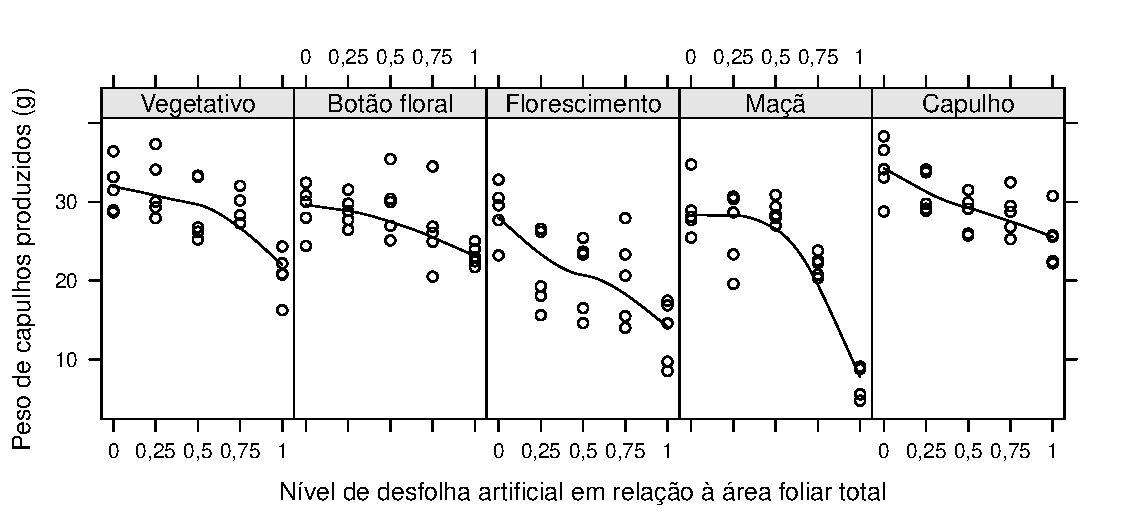
\includegraphics[width=\textwidth]{../figuras/previsu.pdf} 
\end{center}
\caption{Peso de capulhos produzidos (g) em cada estágio fenológico
  como função dos níveis de desfolha artificial. Curvas suaves entre
  os pontos representam as tendências centrais}\label{previsu}
\end{figure} 

Os dados considerados para ajuste do modelo são de um experimento, em
casa de vegetação, com a cultura do algodão (\emph{Gossypium
  hirsutum}). As unidades experimentais foram 2 plantas por vaso para
registro da produção total de pluma com caroço (g).  Os fatores
estudados foram o nível de desfolha artificial (0, 25, 50, 75 e
100\%), feita com tesoura em cada uma das folhas da planta conforme
tais níveis, combinados com o estágio fenológico no qual a desfolha
foi realizada (vegetativo, presença de botão floral, florescimento,
presença de maçã e presença de capulho). O delineamento completamente
ao acaso foi utilizado com cinco repetições, perfazendo $5\times
5\times 5 = 125$ unidades experimentais.  O experimento foi realizado
nas dependências da Universidade Federal de Grande Dourados no ano
agrícola de 2007. Mais informações disponíveis em
\citeonline{Silva2012a}.  Na Figura \ref{previsu} tem se o diagrama de
dispersão dos valores observados de peso de capulhos produzidos (g) em
cada estágio fenológico como função dos níveis de desfolha.

\newpage
\section{RESULTADOS E DISCUSSÃO}

Os ajustes dos modelos aos dados convergiram para os cinco estágios
fenológicos, considerando o máximo de 50 interações.  Valores iniciais
baseados na inspeção do diagrama de dispersão foram considerados
(Figura \ref{previsu}).  As estimativas dos parâmetros comuns,
$\theta_0$ e $\theta_1$, foram idênticas, em termos pontuais e
intervalares, nas duas parametrizações, como de fato devem ser pois
ambas parametrizações descrevem o mesmo modelo (Tabela
\ref{tb-estimic}). Percebeu-se um resultado alarmante para o estágio
de florescimento, no qual os intervalos de confiança para $\theta_0$ e
$\theta_1$ foram demasiado amplos, superando inclusive a amplitude
média de variação dos dados, de aproximadamente 5 g para cima e para
baixo, ao redor da curva de tendência.

\newpage
\section{CONCLUSÕES}

O propósito da reparametrização foi representar o nível de dano
econômico no modelo. As parametrizações foram comparadas com relação
aos métodos disponíveis para fazer inferência sobre o nível de dano
econômico. A inferência baseada em verossimilhança foi mais adequada
no sentido de auxiliar a seleção de modelos. Além do mais,
verificou-se que as medidas de curvatura e inspeção da matriz de
covariâncias das estimativas também são úteis no processo de seleção
de modelos. Nos estágios com pronunciada relação linear para
produção-desfolha, o modelo reparametrizado apresentou melhores
propriedades inferenciais.  O algodoeiro responde de forma
diferenciada à desfolha em cada estágio fenológico.

\newpage
\addcontentsline{toc}{section}{\hspace*{\distnumber}REFERÊNCIAS}
\begin{center}
\section*{REFERÊNCIAS} 
\end{center}


%%.....................................................
%% inclui referências

\begin{flushleft}
\renewcommand\refname{}
\vspace*{-0.9cm}
\begin{singlespace}
\input{../cap3/cap3nls-corrigido.bbl} 
\end{singlespace}
\end{flushleft}

%%.....................................................
%% inclui anexos

\newpage
\addcontentsline{toc}{section}{\hspace*{\distnumber}ANEXOS}
\begin{center}
\section*{ANEXOS} 
\end{center}

\begin{singlespace}
\noindent{{ANEXO A$\,\,$} Código R reproduzível correspondente ao
ajuste do modelo potência reparametrizado para inferência sobre o nível de dano
econômico da desfolha no algodoeiro.
Disponível online
em: \texttt{http://www.leg.ufpr.br/\~{}walmes /TESE/anexoDESF.R}}
\end{singlespace}

\noindent
\lin
\begin{small}
\linespread{0.86}
\input{../scripts/anexoDESF.R}
\lin
\end{small}

\begin{table}
\noindent{{ANEXO B$\,\,$} Peso de capulhos produzido (g) ao final do ciclo a
cada duas plantas de algodão em
  função do nível de desfolha artifical e estágio fenológico.}\\
\begin{center}
 \input{../tabelas/anexotabDESF.txt}
\end{center}
\end{table}


%=========================================================================================================
%333333333333333333333333333333333333333333333333333333333333333333333333333333333333333333333333333333333
% Capítulo 3

\newpage

%% reinicia contadores
\setcounter{section}{0}
\setcounter{figure}{0}
\setcounter{table}{0}
\setcounter{equation}{0}
\renewcommand*{\theHsection}{chY.\the\value{section}}

%% definições de título
\def\titlecapb{Parametrização do modelo van Genuchten para inferência sobre os parâmetros $S$ e $I$}
\def\titlecapB{\expandafter\MakeUppercase\expandafter{\titlecapb}}
\addcontentsline{toc}{section}{\hspace*{\distnumber}CAPÍTULO 3 \titlecapb}

%%.....................................................
%% inclui título

\noindent
\begin{minipage}[t]{0.2\textwidth}
\textbf{CAPÍTULO 3}
\end{minipage}
\begin{minipage}[t]{0.8\textwidth}
\begin{flushleft}
\textbf{\titlecapB} 
\end{flushleft}
\end{minipage}
\vspace{0.8cm}

%%.....................................................
%% inclui resumo e abstract

\begin{center}
\section*{RESUMO} 
\end{center}

\begin{singlespace}
A água é indispensável para produção das culturas pois está envolvida
no transporte de nutrientes, reações químicas, processos físicos e
manutenção da vida do solo. O conhecimento sobre a curva de rentenção
de água (CRA) do solo é fundamental para estabelecer estratégias de
manejo. A qualidade física do solo é depende da CRA e os parâmetros
$I$, tensão do ponto de inflexão da CRA, e $S$, taxa de variação no
ponto de inflexão, considerados como indicadores da qualidade física,
são parâmetros relacionados a medidas descritivas da distribuição do
tamanho de poros do solo. Com este trabalho, objetiva-se verificar o
efeito da posição de amostragem e profundidade do solo sobre os
parâmetros $I$ e $S$ da CRA. Para isso 1) considerou-se ANOVA simples
e 2) ANOVA ponderada pela variância das estimativas desses parâmetros
em cada unidade experimental em comparação com 3) o uso de modelos não
lineares de efeito misto em uma parametrização desenvolvida para $I$ e
$S$. Nenhum dos métodos alternativos de análise foi superior ao modelo
não linear de efeitos mistos na parametrização desenvolvida, que
apresentou intervalos mais estreitos para estimativas dos parâmetros e
apontou efeito de posição e profundidade de coleta nos parâmetros $I$
e $S$.\\
\newline
\noindent {Palavras-chave}: Reparametrização. Função de parâmetros. Método delta. Curva de retenção de água.

\end{singlespace}

\newpage
\begin{center}
\section*{ABSTRACT} 
\end{center}

\begin{singlespace}
Water is essential for crop production because it is involved in the
transport of nutrients, chemical reactions and physical processes
maintaining the soil life. The knowledge about the water retention
curve (WRC) of the soil is important to establish management
strategies. The physical quality of the soil is dependent on the WRC
and the parameters $I$, the inflection point of the WRC, and $S$, the
rate of change at the inflection point, considered as indicators of
quality physical parameters are related to descriptive measures the
pore size distribution of the soil. In this work, we aim to
investigate the effect of sampling position and soil depth on the
parameters $I$ and $S$ of the WRC. For that 1) it was considered ANOVA
and 2) weighted ANOVA based on the variance of these estimates in each
experimental unit compared to 3) using nonlinear mixed-effects in a
parameterization developed for $I$ and $S$. None of the alternative
methods of analysis was superior to the nonlinear mixed effects model
in the parameterization developed, which showed narrower intervals for
parameter estimates and pointed sampling position and depth effect on
parameters $I$ and $S$.\\
\newline
\noindent {Key-words}: Reparametrization. Function of parameters. Delta method. Water retention curve.

\end{singlespace}

%%.....................................................
%% inclui capítulo

\newpage
\section{INTRODUÇÃO}

Água é indiscutivelmente o fator isolado mais importante, com possível
exceção para luz solar e o ar que não têm disponibilidade limitada,
para o desenvolvimento das plantas \cite{Chesworth2007}.  A água
presente no solo desempenha inumeráveis funções de ordem química,
física e biológica como, por exemplo, dissolver e transportar
nutrientes para as plantas além de também ser considerada um nutriente
\cite{Brady2009}.  O excesso de água no solo pode diminuir ou impedir
o desenvolvimento das plantas devido a uma reduzida aeração, enquanto
deficiências podem causar estresse hídrico e, se severa o suficiente,
o murchamento e morte da planta. Para uma produção eficiente, um
fornecimento constante de água é necessário durante o ciclo da planta
para atender as necessidades hídricas e promover a dissolução,
transporte e absorção de nutrientes. O conteúdo de água também
influencia a qualidade de operações de manejo do solo e colheita.

\newpage
\section{RETENÇÃO DE ÁGUA E TAMANHO DE POROS}\label{sc-craporos}

Dada a relação que existe entre tamanho de poros e tensão matricial
é possível chegar à distribuição de frequência
de tamanho de poros quando o modelo \citeonline{VanGenuchten1980} é
usado para representar a CRA \cite{Reynolds2002a}. Essa relação não
pode ser considerada isoladamente pois fatores que alteram as
propriedades da água de um solo para o outro a modificam, como a
concentração de íons e a temperatura. Por outro lado, fixadas as
demais variáveis, essa relação permite explorar a conexão existente
entre a retenção de água e distribuição de tamanho de poros. Além do
mais, a partir dessa relação, é possível verificar que o parâmetro $S$
proposto por \citeonline{Dexter2004} é o parâmetro de escala que
representa o grau de dispersão de valores ao redor do tamanho modal de
poros.

\newpage
\section{MATERIAL E MÉTODOS}\label{sc-methods}

Os dados considerados são medidas de conteúdo de água do solo (m$^3$
m$^{-3}$) em função do potencial matricial (kPa) coletados em campo
sob cultura do cafeeiro no qual se utilizam métodos conservacionistas
e de manejo intensivo do solo \cite{Serafim2011}. Amostras de solo
indeformadas foram coletadas de um solo classificado como Latossolo
Vermelho distroférrico (LVd) em uma lavoura com 3,5 anos de
implantação.

\begin{figure}[!ht]
 \begin{center}
 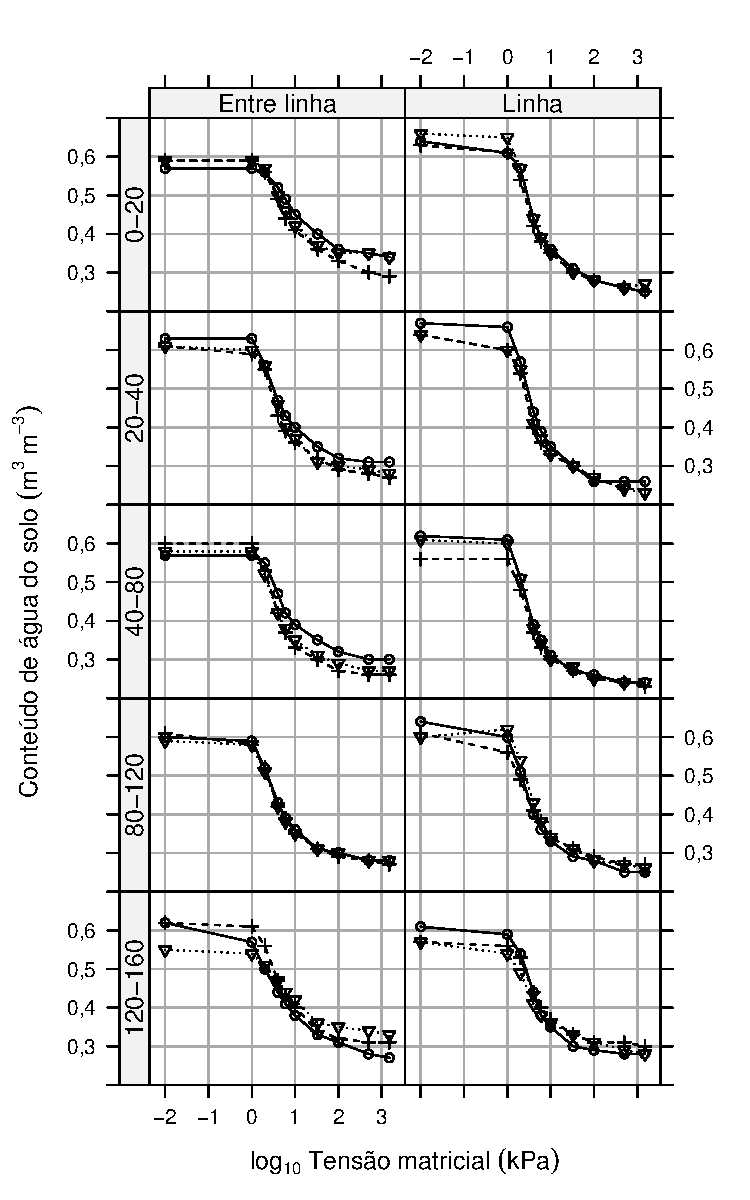
\includegraphics[width=0.7\textwidth]{../figuras/cra_perfil.pdf}
\end{center}
 \caption{Conteúdo de água do solo (m$^3$ m$^{-3}$) em função do
   log$_{10}$ da tensão matricial (kPa) organizado pelas combinações
   entre posição (nas colunas) e profundidade de coleta (nas linhas).
   As três unidades experimentais em cada combinação foram
   identificadas pelos tipos de pontos e linhas}
 \label{fg-craperfil}
\end{figure}

\newpage
\section{RESULTADOS E DISCUSSÃO}\label{sc-results}

Estimativas dos parâmetros foram obtidas para as 30 unidades
experimentais sob as duas parametrizações do modelo van Genuchten.  Os
valores de R$^2$ apontaram boa medida de ajuste pois ficaram entre
98,96\% e 99,88\%.  Pelas estimativas intervalares, considerando os
seis parâmetros definidos pelas duas parametrizações, $U_s$, $U_r$,
$a$, $n$, $S$ e $I$, observamos variação entre unidades experimentais
dentro de uma mesma cela experimental (combinação de posição e
profundidade), entre níveis de profundidade e entre posições de
amostragem (Figura \ref{fg-ICpar}).  Verifica-se que os parâmetros
$U_r$ e $n$, por serem comuns as duas parametrizações, tiveram mesmas
estimativas intervalares independentemente da parametrização.

\begin{figure}[H]
 \begin{center}
 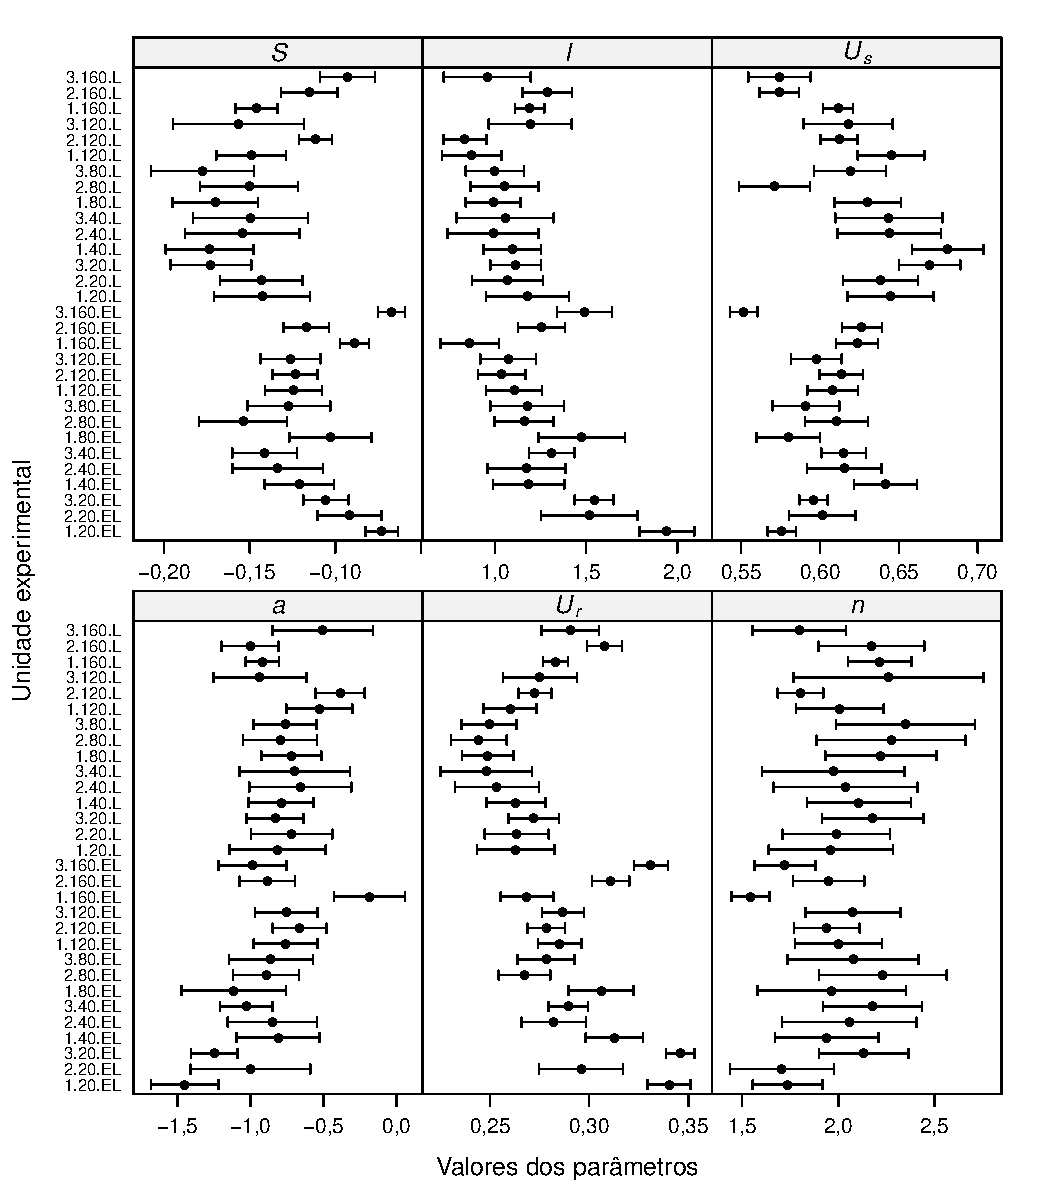
\includegraphics[width=0.8\textwidth]{../figuras/param_ic.pdf}
\end{center}
 \caption{Estimativas intervalares (95\%) pelo método de Wald para os
   parâmetros da CRA considerando as duas parametrizações do modelo
   van Genuchten.  Os rótulos no eixo das coordenadas representam o
   índice da repetição, o nível de profundidade e o nível de posição,
   separados por ponto}
 \label{fg-ICpar}
\end{figure}

\newpage
\section{CONCLUSÕES}\label{sc-conclusion}

Conclui-se que o modelo não linear de efeitos mistos é um método de
análise mais adequado para representar os dados uma vez que toda
informação está contida em um único modelo que permite acomodar os
efeitos de termos fixos e aleatórios, comparar modelos e fazer
predições para a CRA.

\newpage
\addcontentsline{toc}{section}{\hspace*{\distnumber}REFERÊNCIAS}
\begin{center}
\section*{REFERÊNCIAS} 
\end{center}


%%.....................................................
%% inclui referências

\begin{flushleft}
\renewcommand\refname{}
\vspace*{-0.9cm}
\begin{singlespace}
\input{../cap2/cap2nlme-corrigido.bbl} 
\end{singlespace}
\end{flushleft}

%%.....................................................
%% inclui anexos

\newpage
\addcontentsline{toc}{section}{\hspace*{\distnumber}ANEXOS}
\begin{center}
\section*{ANEXOS} 
\end{center}

\begin{singlespace}
\noindent{{ANEXO A$\,\,$} Código R reproduzível correspondente ao
ajuste do modelo van Genuchten reparametrizado. Disponível online
em: \texttt{http://www.leg.ufpr.br/ \~{}walmes/TESE/anexoCRA.R}}
\end{singlespace}

\noindent
\lin
\begin{small}
\linespread{0.86}
\input{../scripts/anexoCRA.R}
\lin
\end{small}

\def\capanexo{Conteúdo de água do solo (m$^3$ m$^{-3}$) em função 
da tensão matricial (kPa), da profundidade (cm) e da unidade 
experimental (UE) para amostras coletadas na}

\begin{sidewaystable}
\noindent{{ANEXO B$\,\,$} \capanexo{} entre linha.}
\begin{center}
 \input{../tabelas/anexotabEL.txt}
\end{center}
\end{sidewaystable}

\begin{sidewaystable}\label{ultima}
\noindent{{ANEXO C$\,\,$} \capanexo{} linha.} \\
\begin{center}
 \input{../tabelas/anexotabL.txt}
\end{center}
\end{sidewaystable}

%% NOTA: \label última em um elemento que esteja na última página é
%% usado para retornar o total de páginas que aparece lá na caixa da
%% ficha catalográfica. Assim não precisa ficar inserindo manualmente.

%=========================================================================================================

\end{document}

%=========================================================================================================
